% ICDE 2027 (Round 2) research-track submission.
% IEEE conference template, <= 12 pages excluding references and the
% AI-generated-content acknowledgement; no appendix; single-blind.
% Numbers are taken from the ACL ARR 2026 submission (Submission 12828), its
% author responses, and the FloodNet measured-byte study (generated/ tables).
% Each number's source is noted in a "% src:" comment next to it.
\documentclass[10pt,conference]{IEEEtran}

\usepackage[T1]{fontenc}
\usepackage[utf8]{inputenc}
\usepackage{microtype}
\usepackage{cite}
\usepackage{graphicx}
\usepackage{booktabs}
\usepackage{multirow}
\usepackage{amsmath,amssymb,amsthm}
\usepackage{algorithm}
\usepackage{algpseudocode}
\usepackage{tikz}
\usetikzlibrary{arrows.meta,positioning,fit,backgrounds}
\usepackage{xspace}
\usepackage{xcolor}
\usepackage{pifont}
\usepackage{comment}
\usepackage[hidelinks]{hyperref}

\DeclareMathOperator*{\argmax}{arg\,max}
\DeclareMathOperator*{\argmin}{arg\,min}
\newcommand{\system}{\textsc{Voila}\xspace}
\newcommand{\R}{\mathcal{R}}
\newcommand{\T}{\mathcal{T}}
\newcommand{\yes}{\ding{51}}
\newcommand{\no}{\ding{55}}
\newcommand{\half}{$\circ$}
\newcommand{\tableformat}{\footnotesize\setlength{\tabcolsep}{3pt}\renewcommand{\arraystretch}{0.95}}
\newtheorem{proposition}{Proposition}
\newtheorem{definition}{Definition}

% Model names (FloodNet tables in the PerCom draft used "Llama-4-Scout" and
% "Qwen2-VL-7B"; inference scripts and the ACL paper use the names below).
\newcommand{\mLlama}{Llama-4-Mav.\xspace}
\newcommand{\mLlava}{LLaVA-1.5-7B\xspace}
\newcommand{\mPix}{Pixtral-12B\xspace}
\newcommand{\mQThree}{Qwen3-VL-235B\xspace}
\newcommand{\mQSevTwo}{Qwen2-VL-72B\xspace}
\newcommand{\mQSev}{Qwen2.5-VL-7B\xspace}

\begin{document}

\title{\system: Query-Driven Representation Selection for\\
VLM Analytics over Multi-Tier Image Data}

% Single-blind review: authors are listed.
\author{
\IEEEauthorblockN{Rahul Atul Bhope\IEEEauthorrefmark{1},
K. R. Jayaram\IEEEauthorrefmark{2},
Vinod Muthusamy\IEEEauthorrefmark{2},\\
Ritesh Kumar\IEEEauthorrefmark{2},
Vatche Isahagian\IEEEauthorrefmark{2},
Nalini Venkatasubramanian\IEEEauthorrefmark{1}}
\IEEEauthorblockA{\IEEEauthorrefmark{1}University of California, Irvine \quad
\IEEEauthorrefmark{2}IBM Research}
}

\maketitle

\begin{abstract}
Data systems increasingly answer natural-language questions over image
collections by invoking vision--language models (VLMs). An image is rarely
stored once. Ingestion pipelines keep a caption, thumbnails, compressed
previews, and the original, spread across device, edge, cloud, and archive
tiers. Yet, typically, a query reads the original from wherever it lives. It pays the
full transfer, retrieval, and inference cost before anyone knows whether that
detail was needed. We argue that choosing \emph{which representation to read}
is a query-optimization decision. A data system should make it before any
pixel is accessed. We present \system, a representation-aware query layer.
\system maintains a representation catalog and learns per-model success
estimators from the query text. It calibrates the estimates so that they are
comparable across representations. It then selects representations per query
or per workload, under byte, latency, and tier-dependent retrieval-cost
objectives and workload budgets. We
evaluate \system on 1,445 disaster-response questions over aerial imagery with
six VLMs (7B--235B parameters). On average, \system is as accurate as the best
fixed representation chosen on validation data (70.5\% vs.\ 70.4\%; per model,
from 1.7 points below to 3.8 points above) while reading 84\% fewer bytes. Compared
with always reading originals, it is 7.3 points more accurate and reads 97.5\%
fewer bytes. Under recorded cellular uplinks, the share of questions answered
correctly within one second rises from 37.9\% to 70.3\%. On VQA-v2, GQA, and
TextVQA, \system reduces tier-weighted access cost by 65--73\% relative to
reading originals, at 1.8--10.6 points lower accuracy. Query-driven selection
also has a clear failure mode. Unseen question templates cost up to 49 accuracy
points. On templated workloads, routing unprofiled templates to a validated
fallback representation recovers the best fixed representation's accuracy.
% src: generated/main_results_table.tex (70.5/70.4, 84%, 97.5%); generated/paired_bootstrap.csv
% (per-model VOILA - best fixed: -1.7..+3.8); tab:breadth (ACL Table 1: cost 35.2/27.9/26.6,
% accuracy -10.1/-10.6/-1.8 vs original); generated_icde/robustness_pooled.csv
\end{abstract}

\begin{IEEEkeywords}
multimodal data management, query optimization, vision--language models,
tiered storage, physical design
\end{IEEEkeywords}

%==========================================================================
\section{Introduction}~\label{sec:intro}

Vision--language models (VLMs) have made it possible to query image collections using natural language. An analyst might ask how many buildings are flooded in an aerial image, an insurer might assess roof damage from a claim photo, or an AI assistant might recall what a sign in a user's photo said. Such queries are increasingly supported by semantic query engines~\cite{patel2024lotus,liu2025palimpzest,jo2024thalamusdb,urban2024caesura}, multimodal retrieval-augmented generation~\cite{lewis2020rag,chen2022murag,yasunaga2023retrievalaugmented}, and agentic memory systems. Despite their different purposes, these systems generally treat an image as a single attribute that is retrieved and passed to a model for interpretation.

\begin{table}[htbp]
\centering
\tableformat
\caption{Fixed-representation accuracy (\%) on the 1,445-question FloodNet
population and measured representation sizes. Bold marks the best fixed
input per model. The original is never the most accurate input; the gap is
significant for every model except \mLlava.}
\label{tab:fixed}
% src: generated/fixed_fidelity_accuracy_table.tex, generated/fidelity_sizes_table.tex
\begin{tabular}{lrrrrr}
\toprule
 & Caption & 32px & JPEG Q1 & JPEG Q10 & Original \\
\midrule
Mean size (bytes) & 281 & 2,141 & 217,576 & 445,479 & 5,520,774 \\
\midrule
\mLlama   & 54.2 & 24.6 & 64.7 & \textbf{70.2} & 63.1 \\
\mLlava   & 73.3 & 73.8 & 42.9 & \textbf{75.6} & 74.7 \\
\mPix     & 17.7 & 20.2 & 28.0 & \textbf{50.5} & 38.8 \\
\mQThree  & 66.0 & 25.8 & 75.9 & \textbf{83.2} & 76.6 \\
\mQSevTwo & 30.7 & \textbf{73.9} & 23.6 & 39.8 & 58.8 \\
\mQSev    & 42.8 & 59.7 & 64.5 & \textbf{71.5} & 67.4 \\
\bottomrule
\end{tabular}
\end{table}

\begin{figure*}[htbp]
  \centering
  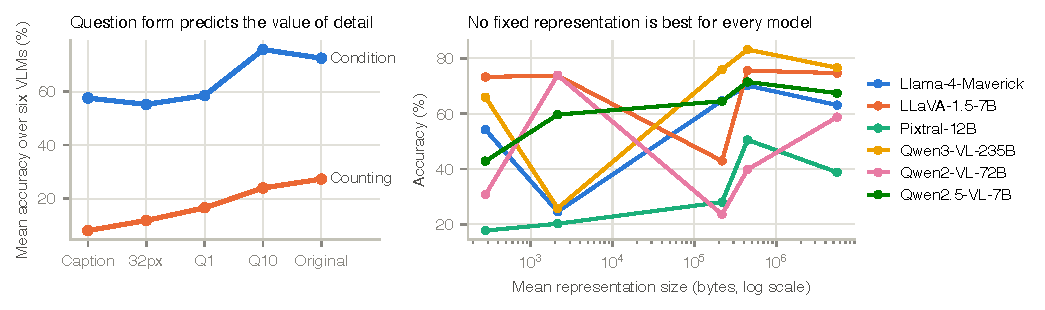
\includegraphics[width=0.95\textwidth]{figures_v2/motivation.pdf}
  \caption{Accuracy by representation on the FloodNet workload. Left:
  questions grouped by surface form and averaged over six VLMs. Counting
  questions benefit from increasing detail, while condition-recognition
  questions peak at a compressed JPEG preview. Right: accuracy is
  non-monotone in representation size, and models differ in their
  preferred input.}
  \label{fig:motivation}
\end{figure*}



This abstraction overlooks how images are stored in practice. Ingestion pipelines often produce multiple representations of the same image, including captions, thumbnails, and compressed previews. These representations can differ in size by four orders of magnitude and may reside on different storage tiers, ranging from device or edge caches to cold object storage and archives~\cite{aws_s3_storage_classes,gcs_storage_classes,azure_blob_storage,lonn2019smartphonepictureorganizationhierarchical}. Different questions, however, require different levels of visual detail. A caption or thumbnail may suffice for some queries, while others require the original image. Yet existing systems often retrieve the original regardless of what the question requires.

This default can be expensive, particularly when the original image must be fetched from a remote or archival storage tier. More surprisingly, it is not always the most accurate choice. For some questions, a smaller representation can produce a better answer than the original image. Section~\ref{sec:usecase} demonstrates both effects using a disaster-response workload.

An alternative is to select a representation based on the question being asked. Existing systems largely leave this decision to the application (\S\ref{sec:gap}), but making it automatically poses two challenges. First, a natural-language question does not explicitly specify the visual detail needed to answer it. Second, the decision must be made before retrieving the image. Inspecting the original to determine which representation is sufficient would defeat the purpose of avoiding that retrieval.

\textbf{Our approach.} We present \system, which makes representation selection a cost-based query optimization decision. Our key observation is that the wording and structure of a question provide a useful prior about the visual evidence needed to answer it (\S\ref{sec:observe}). We use this observation to estimate, from the question alone, the probability that a given VLM will answer correctly using each available representation. These estimates are calibrated separately for each model and representation, and combined with access costs obtained from a representation catalog. The resulting optimizer selects a representation without first retrieving the original image. The same estimates support three optimization problems: per-query selection (P1), workload allocation under a shared budget (P2), and representation placement across storage tiers (P3).

\textbf{Results.} We evaluate \system on 1,445 disaster-response questions using six VLMs. On average, it is as accurate as the best fixed representation chosen on validation data (70.5\% vs.\ 70.4\%) while reading 84\% fewer bytes. Per model, the paired difference ranges from 1.7 points below to 3.8 points above, and is not significant for four of the six models. Under recorded cellular uplinks, it nearly doubles the fraction of questions answered correctly within one second. On three general VQA benchmarks, it reduces tier-weighted access cost by 65--73\% relative to always reading the original, at 1.8--10.6 points lower accuracy (Table~\ref{tab:breadth}). Under shared byte budgets, workload allocation is on average 1.6--3.1 points more accurate than the best fixed representation that fits. In a two-tier simulation, placement guided by the same estimates answers 68.5\% of questions within a 0.25\,s read deadline with 0.5\% of the corpus at the edge, against at most 48.5\% for frequency-based tiering of originals. % src: generated_icde/mission_table.tex (DP 72.2/73.3/73.7 vs best feasible fixed 70.6 at 10/25/50%);
% generated_icde/placement_table.tex (advisor 68.5 at 0.5%; frequency tiering of originals <= 48.5)
Its main weakness is question templates absent from profiling. They cost up to 49 accuracy points, even when worded like profiled ones. On templated workloads, falling back to the best fixed representation recovers that loss.
% src: generated/paired_bootstrap.csv (95% CI includes 0 for Llama, LLaVA, Qwen3, Qwen2-72B; Pixtral +3.8, Qwen2.5-7B -1.7);
% tab:breadth (ACL Table 1); generated_icde/ood/ (TF-IDF cosine >= 0.8 for every held-out template)

\noindent \textbf{Contributions}:
\begin{itemize}
\item We formulate \emph{query-driven representation selection} for VLM queries over multi-representation, multi-tier image data. We study three problems: per-query selection (P1), workload allocation under a shared budget (P2), and representation placement across storage tiers (P3) (\S\ref{sec:model}).

\item We design \system, a representation-aware query layer that combines a representation catalog, calibrated per-model success estimators, and cost-based optimizers. We bound the regret of per-query selection in terms of estimator error and reduce workload allocation to a multiple-choice knapsack problem. For P3 we give a greedy placement advisor rather than an optimal solution (\S\ref{sec:design}).

\item We evaluate \system across six VLMs and four datasets, using measured payload sizes, tier-weighted access costs, recorded network traces, shared workload budgets, and a two-tier placement simulation. Our evaluation uses image-grouped protocols and clustered confidence intervals. We identify cases where fixed representations and supervised routers remain competitive, as well as scenarios where query-driven selection fails (\S\ref{sec:eval}).
\end{itemize}




\section{Motivating Use Case and the Gap}
\label{sec:usecase}

\subsection{Post-disaster damage assessment}

Following a hurricane, survey teams use UAVs to capture high-resolution images of affected neighborhoods~\cite{rahnemoonfar2021floodnet}. Images are captured faster than they can be transferred over degraded networks. They are stored locally on the capture device and copied to a field gateway, which connects to cloud storage over a cellular or satellite backhaul. Over time, the original images may move to colder storage tiers.

Analysts at an emergency operations center query these images to assess damage and plan response efforts. They might ask \emph{``What is the overall condition of this area?''}, \emph{``Is the road flooded?''}, or \emph{``How many buildings are non-flooded?''} Automated agents may issue similar queries, with a cloud-hosted VLM generating the answers.

The FloodNet benchmark~\cite{rahnemoonfar2021floodnet} captures this type of workload. Its questions fall into four classes: condition recognition, yes/no, simple counting, and complex counting. The workload presents competing requirements. Answers must be accurate enough to support response decisions, but they must also arrive quickly. The backhaul is bandwidth-constrained and shared with voice and coordination traffic, while cloud retrieval and VLM inference incur additional costs. The choice of which image representation to retrieve, and from which storage tier, therefore directly affects both response quality and cost.



\subsection{Why fixed representations fall short}

Table~\ref{tab:fixed} shows the five representations available for each FloodNet image, their average sizes, and the accuracy achieved when each VLM uses a fixed representation for every question. The representations range from a 281-byte caption to a 5.5\,MB original image. The results expose the limitations of several straightforward approaches.

\textbf{Always retrieve the original.} This transfers approximately 8\,GB for the 1,445-question workload, or 5.5\,MB per question, and achieves a mean accuracy of 63.2\% across the six models. Under recorded cellular uplinks, only 37.9\% of questions are answered correctly within one second (\S\ref{sec:eval}). Surprisingly, the original is not the most accurate input for any of the six models. A compressed preview or thumbnail performs better in every case, with improvements of up to 15 percentage points. The difference is statistically significant for five of the six models (paired exact McNemar test, $p\le 3\times10^{-4}$). For \mLlava, JPEG Q10 and the original are tied within noise (75.6\% vs.\ 74.7\%, $p=0.28$).
% src: generated_icde/tracker_evidence.txt USE-02 (scripts/tracker_evidence.py)

\textbf{Always retrieve a thumbnail.} A 32px thumbnail is inexpensive to transfer, but its usefulness varies considerably across models. Accuracy ranges from 20.2\% for \mPix to 73.9\% for \mQSevTwo. A representation that works well for one model may perform poorly for another.

\textbf{Escalate when the model is uncertain.} A cascade can begin with a cheap representation and retrieve a more detailed one if the VLM reports low confidence~\cite{chen2023frugalgpt}. This avoids some unnecessary transfers, but incurs additional retrieval and inference costs when escalation is needed. It can also stop prematurely when the model is confident despite missing visual evidence. For \mPix, such a cascade retrieves 1.36\,MB per question and achieves only 44.3\% accuracy (\S\ref{sec:q1}, Table~\ref{tab:main}).

\textbf{Profile each model and fix its best representation.} Choosing each model's most accurate representation on validation data avoids some of these problems. However, it still reads 0.86\,MB per question on average (Table~\ref{tab:main}), because the same representation is retrieved regardless of what the question asks. This is more than the bold entries in Table~\ref{tab:fixed} suggest: those are chosen in hindsight, whereas a validation-based choice sometimes selects the original (for \mLlava and \mQSev). Simple questions incur the cost of representations needed for more demanding ones.
% src: generated/primary_summary.csv (best_fixed mean_bytes, mean 0.857 MB); generated_icde/tracker_evidence.txt USE-01

These results suggest that neither a universal representation nor a fixed choice per model is sufficient. A better approach would select the representation for each question, taking into account both its expected accuracy and retrieval cost. The challenge is to make that decision before accessing the image.

\subsection{What the workload reveals}
\label{sec:observe}



We examine how answer accuracy varies across representations, models, and question types. Three observations motivate our approach.

\textbf{Question form predicts the value of visual detail.}
Figure~\ref{fig:motivation} (left) groups FloodNet questions by their surface form, without examining the underlying images. Averaged across six VLMs, counting questions beginning with \emph{how many} benefit from increasing visual detail. Condition-recognition questions, in contrast, achieve their highest accuracy with a compressed JPEG preview, and some can be answered using captions or thumbnails. We observe similar differences on general VQA workloads. On VQA-v2, yes/no and color questions saturate at JPEG Q10, whereas counting and text-reading questions benefit from the original image.

The important distinction is that these patterns are associated with the question itself. They provide a signal for representation selection that is available before the image is retrieved.

\textbf{More bytes do not necessarily produce better answers.}
Figure~\ref{fig:motivation} (right) shows that accuracy is not monotone in representation size. Larger inputs can perform worse than smaller ones, and the preferred representation differs across VLMs. Representation selection therefore cannot be reduced to choosing the smallest input that approximates the original. It must account for the probability that a particular model will answer correctly using a particular representation.

\textbf{Post-hoc confidence is an unreliable selection signal.}
Cascades typically decide whether to retrieve more detail after processing an initial representation. By then, the system has already incurred retrieval and inference costs. Moreover, model confidence does not reliably indicate whether the available visual evidence is sufficient. On VQA-v2, 43\% of incorrect answers generated from captions have higher log-probability than the median correct answer. For \mQSevTwo, log-probability predicts the need for escalation worse than random (AUC 0.338). We evaluate cascades in \S\ref{sec:q1} and \S\ref{sec:robust}.

Together, these observations point to a different approach: predict the usefulness of each representation directly from the question, rather than inspecting the image or relying on confidence after inference. Because these predictions are model-dependent and uncertain, they must be calibrated before they can support cost-based decisions.



\subsection{The gap in existing systems}
\label{sec:gap}

\begin{table}[htbp]
\centering
\tableformat
\caption{Capabilities needed by the use case. R1: decides before reading
image data (metadata and indexes may be read). R2: ad hoc natural-language queries. R3: multiple representations of an
item. R4: multiple storage tiers. R5: model-specific accuracy estimates. R6:
multi-objective costs and workload budgets. \yes: supported. \half: partially
(\S\ref{sec:gap}). \no: not supported. \system supports R2 only for question
templates seen during profiling (\S\ref{sec:robust}).}
\label{tab:gap}
\begin{tabular}{lcccccc}
\toprule
System class & R1 & R2 & R3 & R4 & R5 & R6 \\
\midrule
VLM APIs and serving~\cite{kwon2023vllm} & \no & \yes & \no & \no & \no & \no \\
Multimodal RAG / vector stores~\cite{lewis2020rag,chen2022murag} & \half & \yes & \no & \no & \no & \no \\
Visual storage managers~\cite{xu2019vstore,haynes2021vss,daum2021tasm} & \yes & \no & \yes & \half & \no & \half \\
ML-inference optimizers~\cite{kang2017noscope,kang2020blazeit,lu2018probabilistic,kang2022tasti,kang2020smol} & \no & \no & \half & \no & \yes & \yes \\
LLM semantic query engines~\cite{patel2024lotus,liu2025palimpzest,jo2024thalamusdb,urban2024caesura} & \no & \yes & \no & \no & \half & \yes \\
Model routers and cascades~\cite{chen2023frugalgpt,chen2020frugalml,wang2024routellm} & \no & \yes & \no & \no & \yes & \half \\
Storage tiering~\cite{aws_s3_intelligent_tiering} & \yes & \no & \no & \yes & \no & \half \\
\midrule
\system & \yes & \half & \yes & \yes & \yes & \yes \\
\bottomrule
\end{tabular}
\end{table}

Several lines of work address parts of this problem, but none jointly considers question-dependent representation accuracy and the cost of accessing representations across storage tiers. Table~\ref{tab:gap} summarizes the capabilities of existing system classes.

\emph{VLM APIs and serving systems} process the inputs provided by the client. They do not generally decide which stored representation should be retrieved. \emph{Multimodal RAG systems and vector stores} focus on identifying which images or documents are relevant to a query. They decide which item to fetch from an index before reading it, but not which form of the item to fetch. They typically retrieve each selected item in a single stored representation, rather than choosing among alternative representations based on the question.

\emph{Visual storage managers} such as VStore, VSS, and TASM~\cite{xu2019vstore,haynes2021vss,daum2021tasm} are closer to our setting. They maintain multiple physical formats or tiles and select inexpensive representations to serve requests. They weigh storage footprint against retrieval cost, but within a single store rather than across tiers, and without workload budgets. However, they generally assume that the consumer specifies its requirements, such as resolution, codec, or region, or that the downstream vision pipeline is fixed and can be profiled in advance. Natural-language questions do not specify these requirements explicitly, and the visual detail needed to answer them depends on both the question and the VLM.

\emph{ML-inference query optimizers}~\cite{kang2017noscope,kang2020blazeit,lu2018probabilistic,kang2022tasti,kang2020smol} use proxy models, sampling, and input-resolution choices to reduce inference costs. Smol~\cite{kang2020smol}, for example, exploits the lower cost of processing small inputs, which is a partial form of representation choice. These approaches generally assume that the underlying visual data is accessible. Their decisions may process image content with inexpensive models, which still reads the data.

\emph{LLM semantic query engines}~\cite{patel2024lotus,liu2025palimpzest,jo2024thalamusdb,urban2024caesura} optimize model choice and operator execution against accuracy and cost targets, but typically treat an image column as a single stored value. Their accuracy estimates are per operator and model, not per input representation. \emph{Model routers and cascades}~\cite{chen2023frugalgpt,chen2020frugalml,wang2024routellm} primarily choose among models or decide whether to invoke a more expensive model. They trade accuracy against model cost, but not under shared workload budgets. They do not address the joint choice of image representation and storage tier, and cascades incur additional retrieval costs when they escalate. Finally, \emph{storage tiering systems}~\cite{aws_s3_intelligent_tiering} place whole objects according to access patterns and storage price rather than the visual evidence required by individual queries.

An application could combine these techniques, but doing so requires substantial additional machinery. It would need to generate and catalog image representations, track their storage locations and access costs, profile VLM accuracy across representations, and predict which inputs are likely to answer each question correctly. It would also need to calibrate those predictions, enforce workload budgets and deadlines, and account for changes in model behavior or question distributions.

The missing component is a query layer that brings these decisions together. This is the role of \system: it uses question-derived estimates of answer correctness and cataloged access costs to select representations before image retrieval, while supporting both individual queries and workload-level optimization.

%==========================================================================



% Editorial revision of Sections 3 and 4.
% Retains the submitted models and measured results; technical issues requiring
% author decisions are tracked in system_paper_todos.md.
%==========================================================================
\section{Data Model and Problem Formulation}
\label{sec:model}

The motivating workload suggests that the representation needed to answer a
question can often be predicted before retrieving the image. We formalize the
assets, costs, and correctness estimates used to make this choice, then define
three optimization problems supported by \system.

\subsection{Multi-representation, multi-tier assets}

An image is an \emph{asset} $x$ with a set of available representations
$\R(x)\subseteq\R$. Our deployment uses five representations:
\[
\R=\{\textit{caption},\textit{thumb}_{32},\textit{jpeg}_{q1},
\textit{jpeg}_{q10},\textit{original}\}.
\]
A materialized instance $(x,r)$ has size $b_r(x)$ and resides at
$\ell(x,r)$ in the tier set
\[
\T=\{\textit{device},\textit{edge},\textit{cloud},\textit{archive}\}.
\]
Representations are derived from the original at ingestion. A
\emph{representation catalog} records each instance's location, size, and
storage pointer, and a pointer to caption text where applicable.
Planning reads catalog metadata, not images.

% TODO MODEL-01: P3 creates tier replicas but the above ell(x,r) permits
% only one tier; decide whether P1 selects (r,t) from an available-copy set.
\subsection{Tiers and cost vectors}

Retrieving representation $r$ of asset $x$ from tier $t$ has cost vector
\[
\mathbf{c}(x,r)=
\big(b_r(x),\;L_t(b_r(x)),\;C_t(b_r(x)),\;I_M(r)\big).
\]
Its components are transferred bytes, access latency, monetary cost, and VLM
inference time. We model access latency as $L_t(b)=\alpha_t+b/\beta_t$,
combining first-byte latency and transfer time. Monetary cost is
$C_t(b)=\kappa_t+\pi_t b$, combining per-request and per-byte charges.
Inference time $I_M(r)$ also depends on the representation: a caption is text,
whereas an image produces visual tokens. A weight vector $\mathbf{w}$ combines
these costs into a scalar objective. Applications may additionally impose hard
constraints, such as a retrieval deadline or spending limit.
% Evaluation scope (inference weight 0, archive not exercised) removed from the model by author, 10 Nov; inference scope stated in Sec. VI-B.

% TODO MODEL-02: Decide whether deadline D should include inference and
% optimizer overhead, rather than only L_t(b).
\subsection{Queries and correctness}

A query $Q=(q,x,M,\mathbf{w},D)$ asks question $q$ about asset $x$ using VLM
$M$, under weights $\mathbf{w}$ and deadline $D$. Let
$Y_r(q,x)\in\{0,1\}$ indicate whether $M$ answers correctly using
representation $r$. This outcome is not known when the optimizer makes its
decision. Instead, it estimates
\begin{equation}
 p_r(q)=\Pr\big[Y_r(q,x)=1\mid\phi(q)\big],
 \label{eq:success}
\end{equation}
where $\phi(q)$ contains features extracted from the question and, optionally,
precomputed catalog statistics. The estimator does not read a representation
of $x$. The probability describes expected success over the workload, not a
guarantee for an individual image.

\subsection{Three optimization problems}

\begin{definition}[\textbf{P1: Per-query selection}]
Given $Q$ and estimates $\widehat p_r$, choose
\begin{equation}
 r^*(Q)=\arg\max_{r\in\R(x):\,L_{\ell(x,r)}(b_r(x))\le D}
 \big[\widehat p_r(q)-\lambda\,\mathbf{w}^\top\mathbf{c}(x,r)\big].
 \label{eq:p1}
\end{equation}
\end{definition}

The objective values a correct answer at one unit and trades expected
correctness against weighted access and inference costs. Selecting $r$ incurs
the cost of that representation alone, rather than the cumulative cost of all
smaller representations. This distinguishes direct selection from a cascade.

\begin{definition}[\textbf{P2: Workload allocation}]
Given a batch $\mathcal{Q}$ and a budget $B$ on scalar cost
$c=\mathbf{w}^\top\mathbf{c}$, choose one representation $r(Q)$ for each query
to maximize $\sum_{Q\in\mathcal{Q}}\widehat p_{r(Q)}$, subject to
$\sum_{Q\in\mathcal{Q}}c(x_Q,r(Q))\le B$.
\end{definition}

\begin{definition}[\textbf{P3: Representation placement}]
Given a workload distribution $\mathcal{W}$, tier capacities $K_t$, and
per-tier cost models, choose which asset--representation instances to
materialize on each tier. The placement maximizes expected P1 utility for
$\mathcal{W}$ subject to the storage capacity of each tier.
\end{definition}

\textbf{P1} handles queries as they arrive. \textbf{P2} allocates a shared budget across a known
batch, as when a response mission has a fixed backhaul allowance. \textbf{P3} is an
offline physical-design problem, analogous to materialized-view and index
selection~\cite{harinarayan1996cubes,chaudhuri1997autoadmin}. We do not solve P3
optimally; \S\ref{sec:design} gives a greedy placement advisor, which we evaluate in a
two-tier simulation. The same
correctness estimates used at query time also score candidate placements.

% TODO MODEL-01: Reinstate a precise set/capacity formulation for P3 once
% replica semantics and the asset dimension are resolved.
\subsection{Guarantees}

The quality of P1 depends on estimation error. The following bound makes this
dependence explicit.

\begin{proposition}[Selection regret]
\label{prop:regret}
For query $Q$, let
$\epsilon(Q)=\max_r|\widehat p_r(q)-p_r(q)|$ over feasible representations.
Let $r^*$ maximize the true objective in~\eqref{eq:p1}, and let $\widehat r$
maximize the estimated objective over the same feasible set. Then the utility
lost by choosing $\widehat r$ is at most $2\epsilon(Q)$. The expected regret
is therefore at most $2\,\mathbb{E}_Q[\epsilon(Q)]$.
\end{proposition}

\begin{proof}
Add and subtract the estimated utilities of $r^*$ and $\widehat r$. The
difference between their estimated utilities is non-positive because
$\widehat r$ maximizes that objective. Each of the remaining two terms is
bounded by $\epsilon(Q)$; the cost terms cancel because the same costs are
used in both objectives. Taking expectations gives the second claim.
\end{proof}

The guarantee relates selection regret to the estimator's error on the
operating workload. It does not bound error uniformly across unseen query
distributions or establish a finite-sample guarantee for calibration. We
therefore use disjoint populations for estimator training, calibration, and
operating-point selection (\S\ref{sec:design}).

P2 is a multiple-choice knapsack problem (MCKP). Each query is a class and
each representation is an item, with value $\widehat p_r$ and cost $c$.
Although MCKP is NP-hard, its LP relaxation can be solved by considering
incremental value per cost on the upper convex hull of each class. An optimal
basic LP solution has at most one fractional class~\cite{sinha1979mckp}.
Provided the cheapest allocation is feasible, rounding that class down loses
at most one expected correct answer relative to the integer optimum, since
$0\le\widehat p_r\le1$. This gives a useful bound for large batches.

% TODO MODEL-03: Verify the LP/rounding statement and assumptions against
% the cited result and distinguish it from the bucketed-DP implementation.
%==========================================================================
\section{\system Design}
\label{sec:design}

\begin{figure*}[t]
\centering
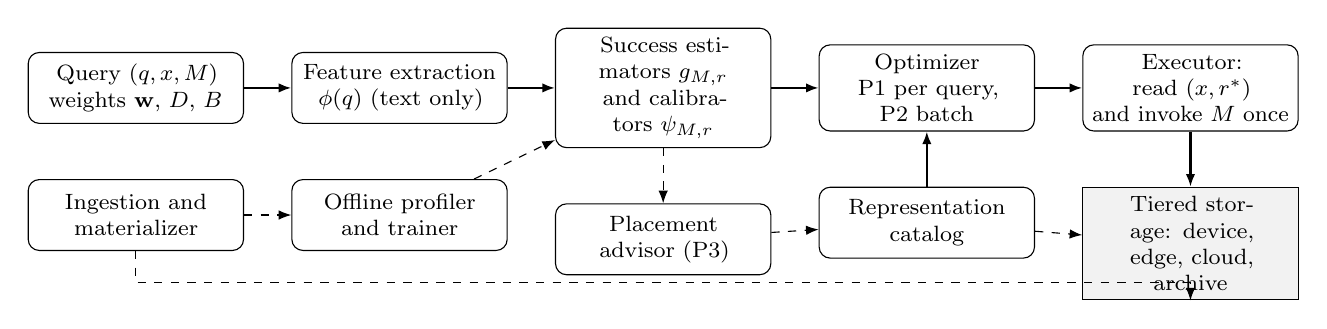
\begin{tikzpicture}[
 font=\footnotesize,
 box/.style={draw,rounded corners,align=center,minimum height=9mm,text width=25mm,fill=white},
 store/.style={draw,align=center,minimum height=9mm,text width=25mm,fill=gray!10},
 arrow/.style={-{Latex[length=1.6mm]},thick},
 darrow/.style={-{Latex[length=1.6mm]},dashed},
 node distance=7mm and 6mm]
\node[box] (q) {Query $(q,x,M)$\\weights $\mathbf{w}$, $D$, $B$};
\node[box,right=of q] (feat) {Feature extraction\\$\phi(q)$ (text only)};
\node[box,right=of feat] (est) {Success estimators $g_{M,r}$\\and calibrators $\psi_{M,r}$};
\node[box,right=of est] (opt) {Optimizer\\P1 per query, P2 batch};
\node[box,right=of opt] (exec) {Executor: read $(x,r^*)$\\and invoke $M$ once};
\node[box,below=of q] (ing) {Ingestion and\\materializer};
\node[box,below=of feat] (prof) {Offline profiler\\and trainer};
\node[box,below=of est] (place) {Placement\\advisor (P3)};
\node[box,below=of opt] (cat) {Representation\\catalog};
\node[store,below=of exec] (tiers) {Tiered storage: device,\\edge, cloud, archive};
\draw[arrow] (q)--(feat);
\draw[arrow] (feat)--(est);
\draw[arrow] (est)--(opt);
\draw[arrow] (opt)--(exec);
\draw[arrow] (cat)--(opt);
\draw[arrow] (exec)--(tiers);
\draw[darrow] (ing)--(prof);
\draw[darrow] (prof)--(est);
\draw[darrow] (est)--(place);
\draw[darrow] (place)--(cat);
\draw[darrow] (cat)--(tiers);
\draw[darrow] (ing.south) -- ++(0,-4mm) -| (tiers.south);
\end{tikzpicture}
\caption{\system architecture. The solid path performs query-time selection
using the question and catalog metadata; only the executor reads a
representation. Dashed arrows show offline ingestion, profiling, and
placement.}
\label{fig:arch}
\end{figure*}

Figure~\ref{fig:arch} shows the online and offline components of \system.
At query time, the system extracts text features, estimates the probability
of a correct answer for each available representation, and combines those
estimates with cataloged access costs. The executor then retrieves the chosen
representation and invokes the target VLM once. Separately, ingestion creates
representations, profiling trains and calibrates the estimators, and a
placement advisor determines which tiers should hold them.

\subsection{Query interface and catalog}

\system exposes representation selection as an access-path choice for a VLM
operator. Consider a semantic query:
\begin{center}
\footnotesize
\begin{tabular}{l}
\texttt{SELECT a.id, ASK(a.image, 'How many buildings}\\
\texttt{\ \ are flooded?', 'qwen3-vl') FROM aerial a}\\
\texttt{WHERE a.sector = 4}\\
\texttt{WITH (accuracy\_floor = 0.95, deadline = 1s)}
\end{tabular}
\end{center}

Here \texttt{a.image} denotes an asset, rather than its bytes. The query
planner leaves the representation passed to \texttt{ASK} unresolved. For each
qualifying asset, \system uses the question and catalog metadata to choose a
representation before retrieving the image. The executor can group these
reads by tier, while P2 can allocate a shared budget across the qualifying
queries. This decision can also be inserted into an existing semantic query
engine~\cite{patel2024lotus,liu2025palimpzest}: \system chooses the input
representation, leaving operator ordering and model selection to the host
engine.

The representation catalog has schema
\begin{center}
\footnotesize
\begin{tabular}{l}
\texttt{Rep(asset\_id, rep, tier, uri, bytes,}\\
\texttt{\ \ derived\_from, created\_at, caption\_text\_uri)}
\end{tabular}
\end{center}
and stores one row per materialized instance. Tier parameters
$(\alpha_t,\beta_t,\kappa_t,\pi_t)$ are maintained separately. Changes in
prices or measured bandwidth update cost estimates without retraining the
success estimators. Each target VLM also has a profile containing its
representation estimators, calibrators, validated operating point, and label
provenance. Since planning requires only metadata and model profiles, the
catalog can be replicated at the edge or on devices.

% TODO DESIGN-01: The example's accuracy_floor=0.95 must be aligned with
% the actual relative validation floor of 0.95*A_fix.
% TODO MODEL-01: If replicas are permitted, Rep's key must include tier.
\subsection{Ingestion and materialization}

The materializer generates representations where the original is first
available. It creates thumbnails and JPEG previews by re-encoding the image,
and uses a captioning model to generate a caption. Captioning is performed
once per asset, so its creation cost is amortized over subsequent queries.
Our online cost accounting excludes that one-time cost, which we did not
measure; we also evaluate \system without captions (\S\ref{sec:robust}). The materializer records the
size and location of each resulting representation in the catalog.

\subsection{Offline profiling}

For each target VLM $M$, profiling runs the model on labeled questions at
every representation and records the correctness outcome $Y_r$. This is the
only stage in the design that deliberately evaluates multiple representations
for the same question. The resulting labels are used to train the success
estimators. Each outer fold's training questions are split by group into 70\%
for the estimators, 15\% for calibration, and 15\% for operating-point
selection; on FloodNet this leaves 1,156 labeled questions per fold. Fitting
all five estimators and calibrators takes 0.5\,s on FloodNet and 41\,s on
12,000 VQA-v2 questions on one laptop CPU (Apple M4).
% src: VOILA_code scripts/run_all_experiments.py L1457-1474 (70/15/15 split, leakage asserts);
% generated_icde/planner_overhead.txt (scripts/planner_overhead.py, own re-implementation, same hyperparameters)

\subsection{Success estimators}

The input to each estimator is a feature vector $\phi(q)$ built from the
question text. It contains sparse TF--IDF features and structural indicators,
including counting expressions, yes/no auxiliaries, numerals, negation,
superlatives, and question length. For each model--representation pair
$(M,r)$, a gradient-boosted estimator $g_{M,r}$ predicts a raw success score.
The estimators learn from the model's observed correctness labels; they do not
inspect image content at query time.

The estimator family is replaceable. With calibration and the optimizer held
fixed, gradient boosting, logistic regression, ridge regression, and an MLP
differ by at most 1.6 accuracy points for \mPix on VQA-v2, and a fine-tuned
BERT regressor in the same pipeline does not consistently improve the
accuracy--cost trade-off (both in \S\ref{sec:robust}). We use gradient
boosting because it has low training and prediction overhead in this setting.
The interface also permits features computed at ingestion and recorded in the
catalog, such as representation sizes. We do not rely on such features for the
reported question-text-only results.
% TODO E3: Evaluate catalog-statistic features; do not imply a completed result.

\subsection{Per-representation calibration}

Raw estimator scores are not directly comparable: a score of 0.6 for a
caption need not imply the same success probability as 0.6 for the original.
Because the optimizer trades estimated correctness against cost, these scores
must be calibrated. For each $(M,r)$, \system fits an isotonic map
$\psi_{M,r}$ on a population disjoint from estimator training (the 15\%
calibration split), producing
\[
\widehat p_r(q)=\psi_{M,r}\big(g_{M,r}(\phi(q))\big).
\]
We calibrate each representation separately and do not require correctness to
increase with representation size; Table~\ref{tab:fixed} shows why such a
constraint would be inappropriate.

\subsection{Per-query optimizer}

Algorithm~\ref{alg:p1} implements P1. Using catalog metadata, it excludes
representations that are unavailable for the asset or violate the retrieval
deadline. It evaluates the lightweight estimators for the remaining
candidates, computes their expected utilities, and selects the maximizer. The
online path reads one representation and invokes the VLM once, rather than
retrieving progressively larger inputs. Planning a query takes 0.64\,ms
(median; 7\,$\mu$s per query when batched) on one laptop CPU core, which is
small next to the access latencies of \S\ref{sec:objectives}.
% src: generated_icde/planner_overhead.txt (scripts/planner_overhead.py)

The operating-point parameter $\lambda$ is selected on validation data,
separate from both training and calibration. Let
$A^{\mathrm{val}}_{\mathrm{fix}}$ be the accuracy of the best fixed
representation on that population. Among candidate penalties achieving at
least $0.95A^{\mathrm{val}}_{\mathrm{fix}}$, \system selects the one that
transfers the fewest bytes. This is a relative validation accuracy target,
not a per-query guarantee; applications may choose a stricter trade-off.

Unlike sequential escalation, P1 compares the full utility of each available
representation. An earlier incremental-gain heuristic remains in the
experimental ablations, but does not implement the P1 objective.

\begin{algorithm}[t]
\caption{Per-query representation selection (P1)}
\label{alg:p1}
\begin{algorithmic}[1]
\Require query $(q,x,M)$, weights $\mathbf{w}$, deadline $D$, penalty $\lambda$
\State $F\gets\{r\in\R(x): L_{\ell(x,r)}(b_r(x))\le D\}$ \Comment{catalog only}
\If{$F=\emptyset$}
  \State $F\gets\{\arg\min_{r\in\R(x)}L_{\ell(x,r)}(b_r(x))\}$
  \Comment{best effort; deadline unmet}
\EndIf
\ForAll{$r\in F$}
  \State $\widehat p_r\gets\psi_{M,r}(g_{M,r}(\phi(q)))$
  \State $u_r\gets\widehat p_r-\lambda\,\mathbf{w}^\top\mathbf{c}(x,r)$
\EndFor
\State $r^*\gets\arg\max_{r\in F}u_r$
\State Read $(x,r^*)$ from $\ell(x,r^*)$; \Return $M(q,(x,r^*))$
\end{algorithmic}
\end{algorithm}

% TODO DESIGN-02: Decide if best-effort deadline violation is permitted
% by the API; otherwise explicitly return infeasible.
\subsection{Workload optimizer}

For a known batch with a shared budget, \system solves P2 as an MCKP: each
query contributes one class, with a candidate item for each representation.
We implement two allocators. \emph{Bucketed dynamic programming} rounds costs
up to 1\,KiB buckets and retains Pareto-optimal (cost, value) states. Rounding
up makes the returned allocation feasible under the unrounded budget, though
it need not be optimal for the original continuous-cost instance. In our
measurements, a 100-query batch is solved in under a second.
\emph{Marginal-value allocation} is a greedy alternative: it initially assigns
each query its cheapest representation, then applies upgrades in decreasing
order of predicted accuracy gain per additional unit cost, provided they fit
within the remaining budget.
% src: VOILA_code scripts/percom_experiments.py mckp_dynamic_program, greedy_upgrades

Both methods plan over a batch; single queries use P1.

\subsection{Placement advisor}
\label{sec:advisor}

P3 uses the same correctness estimates to guide representation placement.
For a candidate placement, the placement advisor replays a sample of the workload
through the P1 decision rule, restricted to representations available at the
modeled tiers. It measures the expected utility under that placement. Starting
from representations stored in the cloud, it greedily copies the
asset--representation instance with the largest popularity-weighted utility
gain per added storage byte to a faster tier, stopping at the tier's capacity.
Popularity weights come from the expected workload. The cloud copy is
retained, and P1 reads the fastest available copy. A copy can improve utility
by lowering a tier-dependent cost or by making a representation feasible
under a deadline. With the byte objective we evaluate, cost does not depend on
the tier, so all of the placement advisor's measured gains come from deadline
feasibility. Placement evaluation uses the success estimators rather than
invoking VLMs, so the placement advisor scores every (image, representation) candidate,
7,225 on FloodNet, offline (\S\ref{sec:placement-eval}).

% TODO MODEL-01: The P1 equations and catalog must support selecting among
% multiple copies of the same representation for this advisor to be exact.
% TODO DESIGN-03: Reconcile cloud-at-ingestion initial placement with
% on-device/edge materialization and originals aging into archive.
\subsection{Maintenance}

\textbf{New representations.} Since estimators are defined per
model--representation pair, adding a representation requires profiling and
training its estimator and calibrator; existing representation estimators do
not need to be retrained.

\textbf{New models.} Estimators trained on an earlier model can provide a
starting point for a newer one, with recalibration as new labels become
available. Within the Qwen family, zero-shot transfer is 3.4--4.5 accuracy
points below a target-trained estimator on VQA-v2 and matches its accuracy on
GQA (\S\ref{sec:robust}).

\textbf{Unseen question forms.} Question-text estimators are less reliable on
templates absent during profiling (\S\ref{sec:robust}). For workloads drawn
from a fixed set of question templates, as in FloodNet, the model profile
records the normalized question strings (lowercase, punctuation removed) seen
during profiling. A query whose string is not recorded reads the best fixed
representation on the profiling data until labels for its template are
collected. Because matching is exact, a rephrased profiled question is also
treated as new. That forgoes savings on the query but avoids the held-out
template failure. A feature-distance test does not work: every held-out
FloodNet template has TF--IDF cosine similarity of at least 0.8 to a profiled
one (\S\ref{sec:robust}). Exact matching does not suit open-ended workloads.
On VQA-v2, GQA, and TextVQA, 69--82\% of test questions have a string never
seen in training, so the fallback would disable selection for most queries.
We do not use it on those workloads.
% src: generated_icde/template_coverage.txt (scripts/template_coverage.py); generated_icde/ood/
% DESIGN-08 (was DESIGN-04) resolved 10 Nov; false negatives cannot occur with exact matching,
% false positives (rephrasings) are unmeasured because FloodNet has none.



%==========================================================================
\section{Experimental Setup}
\label{sec:setup}

\textbf{Primary workload.} We use the FloodNet visual question answering
benchmark~\cite{rahnemoonfar2021floodnet} as the disaster-response workload.
The common population contains 1,445 questions. For each, all five
representations and the outputs of all six VLMs are available. We report
measured payload bytes per representation (Table~\ref{tab:fixed}). Each of five
outer folds holds out images, not questions. The remaining images are split
into disjoint populations for estimator training (70\%), calibration (15\%),
and operating-point validation (15\%). Questions about the same image therefore never
cross a boundary. Confidence intervals and paired differences resample image
clusters, with 2,000 bootstrap replicates.

\textbf{Breadth workloads.} To test generality, we also use VQA-v2, GQA, and
TextVQA~\cite{goyal2017vqav2,hudson2019gqa,singh2019textvqa}. These runs use a
tier-weighted cost, normalized so that reading the original costs 100. The
other costs are 7.6 (caption), 15.1 (thumbnail), 37.8 (JPEG Q1), and 53.2 (JPEG
Q10). They are derived from measured size ratios and a base cost per tier
(edge, warm, cold). These runs use question-level five-fold cross-validation.
We also report an image-grouped re-run.

\textbf{Models.} We use \mPix~\cite{pixtral2024}, \mLlama~\cite{meta2025llama4},
\mLlava~\cite{liu2024improved}, \mQSevTwo~\cite{Qwen2VL},
\mQSev~\cite{bai2025qwen25vl}, and \mQThree~\cite{qwen3vl2025}. All run
zero-shot. They span 7B to 235B parameters.

\textbf{Baselines.} \emph{Fixed} always reads one representation. \emph{Best
fixed} is the fixed representation with the highest validation accuracy in
each fold. \emph{Log-prob cascade} is a FrugalGPT-style
cascade~\cite{chen2023frugalgpt}. It reads representations in increasing size.
It stops when the VLM's answer log-probability exceeds a validation-tuned
threshold. Its cost is cumulative. \emph{BERT router} is a supervised
sentence-embedding classifier that predicts the cheapest correct
representation. \emph{GPT-4o router} (breadth only) has GPT-4o label each
question's visual need as low, medium, or high. \emph{Oracle} picks the
cheapest representation that answers correctly, in hindsight.

\textbf{Metrics.} We report accuracy and mean bytes per query (FloodNet) or
normalized cost (breadth). Under recorded network traces we report
deadline-qualified accuracy (DQA), the probability that an answer is correct
and its read finishes within deadline $D$:
$\mathrm{DQA}(D)=\Pr[Y=1\wedge T_{\mathrm{access}}\le D]$. For workloads, we
report accuracy under a shared batch budget.



%==========================================================================
\section{Evaluation}
\label{sec:eval}

We ask five questions. (Q1) Does query-driven selection improve the
accuracy--cost frontier over fixed and adaptive policies? (Q2) Do the gains
hold under other cost objectives? (Q3) How should a workload budget be
allocated? (Q4) What do selections imply for placement? (Q5) How robust and
maintainable is \system, and where does it fail?

\subsection{Q1: Per-query selection}
\label{sec:q1}

\begin{table}[t]
\centering
\tableformat
\caption{FloodNet accuracy (\%) and measured MB per query. Best fixed is
chosen on validation data. Cascade bytes are cumulative.}
\label{tab:main}
% src: generated/main_results_table.tex
\resizebox{\columnwidth}{!}{%
\begin{tabular}{lrrrrrrrrrr}
\toprule
 & \multicolumn{2}{c}{Original} & \multicolumn{2}{c}{Best fixed} &
 \multicolumn{2}{c}{Cascade} & \multicolumn{2}{c}{BERT} &
 \multicolumn{2}{c}{\system} \\
Model & Acc & MB & Acc & MB & Acc & MB & Acc & MB & Acc & MB \\
\midrule
\mLlama   & 63.1 & 5.52 & 69.2 & 0.400 & 52.4 & 0.120 & 72.5 & 1.000 & 68.2 & 0.087 \\
\mLlava   & 74.7 & 5.52 & 74.9 & 2.386 & 73.1 & 0.047 & 76.5 & 0.903 & 75.7 & 0.015 \\
\mPix     & 38.8 & 5.52 & 50.5 & 0.445 & 44.3 & 1.364 & 53.0 & 1.384 & 54.3 & 0.242 \\
\mQThree  & 76.6 & 5.52 & 83.2 & 0.445 & 67.3 & 0.052 & 82.5 & 1.120 & 82.1 & 0.113 \\
\mQSevTwo & 58.8 & 5.52 & 73.9 & 0.002 & 70.3 & 0.910 & 40.9 & 0.756 & 73.3 & 0.002 \\
\mQSev    & 67.4 & 5.52 & 70.9 & 1.461 & 60.1 & 0.487 & 70.3 & 1.641 & 69.2 & 0.358 \\
\midrule
Mean      & 63.2 & 5.52 & 70.4 & 0.857 & 61.3 & 0.497 & 66.0 & 1.134 & 70.5 & 0.136 \\
\bottomrule
\end{tabular}}
\end{table}

\begin{figure*}[t]
\centering
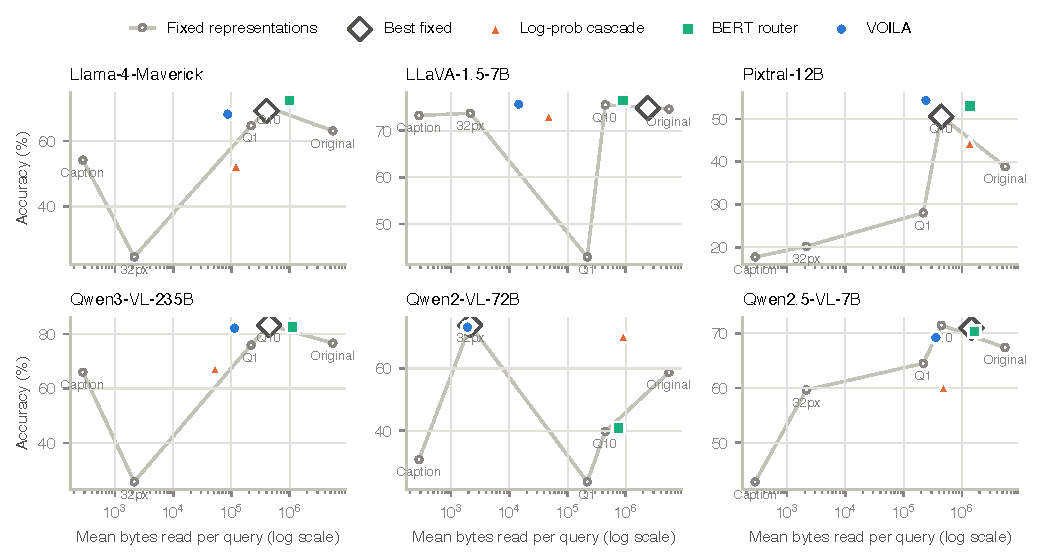
\includegraphics[width=0.95\textwidth]{figures_v2/frontier.pdf}
\caption{Accuracy versus measured bytes on FloodNet. Every point uses the same
image-grouped test population. Fixed points trace the five representations.
Cascade points include every representation read before stopping.}
\label{fig:frontier}
\end{figure*}

\textbf{\system reaches best-fixed accuracy at a fraction of the bytes.}
Table~\ref{tab:main} and Figure~\ref{fig:frontier} show the results. \system
averages 70.5\% accuracy at 0.136\,MB per query. The best fixed representation
averages 70.4\% at 0.857\,MB, and it requires knowing in advance which
representation suits each model. Reading originals averages 63.2\% at
5.52\,MB. \system is thus as accurate as the best fixed policy while reading
84\% fewer bytes. It is 7.3 points more accurate than reading originals while reading
97.5\% fewer bytes.

\textbf{The gain is model-dependent.} We compare \system with best fixed using
paired, image-clustered resampling. \system is more accurate by 3.8 points on
\mPix and by 0.8 points on \mLlava. It is less accurate by 0.6--1.7 points on
the other four models. It reads fewer bytes in every case.
% src: generated/paired_results_table.tex
For \mQSevTwo, best fixed is the 32-pixel thumbnail. \system reads 1,916 bytes
per query against the thumbnail's 2,141 and is 0.6 points less accurate.
Neither policy dominates. The 95\% confidence intervals on \system's accuracy
span 4--5 points per model. Those on its bytes are narrow (e.g., \mQThree:
0.103--0.122\,MB). The byte savings are therefore not driven by a few large
originals.

\textbf{Supervised routing is more accurate on some models but reads far
more.} The BERT router is 4.2 points more accurate than \system on \mLlama. It
reads 1.13\,MB per query on average, 8$\times$ more than \system. On
\mQSevTwo it collapses to 40.9\%. It predicts a label (the cheapest correct
representation) rather than comparable probabilities. It therefore has no way
to trade accuracy against cost.

\textbf{Cascades pay for confidence they cannot trust.} The log-prob cascade
is cheaper than \system on some models. It sacrifices up to 14.8 points in
doing so (\mQThree: 67.3\% vs.\ 82.1\%). On \mPix it reads 1.36\,MB per query
and reaches 44.3\%, worse than \system on both axes.

\textbf{The same holds across datasets.} Table~\ref{tab:breadth} reports the
breadth workloads under tier-weighted cost. \system reduces cost by 65--73\%
relative to originals. On TextVQA it is within 1.8 points of the original at
27\% of its cost. On VQA-v2 and GQA, the accuracy gap to the original is 10.1
and 10.6 points. A fixed JPEG Q10 preview is more accurate than \system on these
two datasets, but it costs 51--91\% more. \system dominates the log-prob cascade
on all three datasets. It dominates the BERT router on VQA-v2 and TextVQA. On
GQA it ties the BERT router (59.6\% vs.\ 59.7\%) at 32\% lower cost. The GPT-4o
router is more accurate on VQA-v2. It costs 40\% more and requires a
large-model call per query.

\begin{table}[t]
\centering
\tableformat
\caption{Breadth workloads: mean accuracy (\%) / normalized tier-weighted cost
(original $=100$) over six VLMs. JPEG Q10 is the strongest fixed preview.}
\label{tab:breadth}
% src: ACL Table 1; JPEG Q10 row averaged from ACL Table 4.
\begin{tabular}{lccc}
\toprule
Policy & VQA-v2 & GQA & TextVQA \\
\midrule
Caption            & 47.8 / 7.6  & 39.9 / 7.6  & 75.7 / 7.6 \\
JPEG Q10           & 72.0 / 53.2 & 67.0 / 53.2 & 81.3 / 53.2 \\
Original           & 75.0 / 100  & 70.2 / 100  & 86.6 / 100 \\
Log-prob cascade   & 54.5 / 36.6 & 51.1 / 44.7 & 71.9 / 39.3 \\
GPT-4o router      & 67.2 / 49.2 & 57.7 / 40.5 & 84.5 / 70.7 \\
BERT router        & 62.0 / 40.9 & 59.7 / 40.9 & 71.9 / 33.1 \\
\system            & 64.9 / 35.2 & 59.6 / 27.9 & 84.8 / 26.6 \\
\midrule
Oracle (hindsight) & 86.9 / 29.8 & 83.5 / 33.2 & 96.7 / 18.2 \\
\bottomrule
\end{tabular}
\end{table}

\subsection{Q2: Cost objectives beyond bytes}
\label{sec:objectives}

\textbf{Latency under recorded networks.} We replay six public CellReplay
uplink traces~\cite{cellreplay-nsdi25}. They cover two carriers and driving,
stationary, weak-signal, crowded, and walking scenarios. We treat each recorded
delivery opportunity as a 1,400-byte slot and sample 100 start phases per
query. Table~\ref{tab:trace} reports serialization latency and deadline-qualified
accuracy (DQA, \S\ref{sec:setup}), averaged
over models and scenarios. Reading originals completes within one second for
59.3\% of queries. Its one-second DQA is 37.9\%. \system completes 99.7\% of
reads within one second and reaches 70.3\% DQA. Its p95 access latency is
0.23\,s, versus 2.96\,s for originals. A deadline-aware best fixed policy
matches \system's DQA. It reads 2.6$\times$ the bytes and has a higher p95
latency. The DQA gap to originals persists in every scenario. In the
weak-signal trace, no original arrives within one second. \system answers
69.8\% of questions correctly in time.
% src: generated/trace_results_table.tex, trace_scenario_table.tex

\begin{table}[t]
\centering
\tableformat
\caption{Recorded-trace access latency (s) and deadline-qualified accuracy
(\%), averaged over six VLMs and six uplink scenarios. C@1: fraction of reads
completing within 1\,s.}
\label{tab:trace}
% src: generated/trace_results_table.tex
\begin{tabular}{lrrrrrr}
\toprule
Policy & MB & p50 & p95 & C@1 & DQA@1 & DQA@10 \\
\midrule
Original    & 5.521 & 1.428 & 2.959 & 59.3 & 37.9 & 63.0 \\
Best fixed  & 0.359 & 0.112 & 0.281 & 99.5 & 70.3 & 70.8 \\
Cascade     & 0.497 & 0.034 & 1.237 & 96.3 & 59.7 & 61.2 \\
BERT router & 1.134 & 0.054 & 2.370 & 91.7 & 63.6 & 65.9 \\
\system     & 0.136 & 0.052 & 0.230 & 99.7 & 70.3 & 70.5 \\
\bottomrule
\end{tabular}
\end{table}

\textbf{Tier-weighted access cost.} The breadth results in
Table~\ref{tab:breadth} already price representations by tier, not by bytes
alone. Captions and thumbnails are served from an edge tier. Previews come
from a warm tier, and originals from a cold tier. P1 depends only on cost
differences. Rescaling or shifting costs while preserving their order
therefore leaves the per-query decision unchanged for a fixed cost weight
$\lambda$ (Eq.~\ref{eq:p1}). Only the operating point moves.

\textbf{Inference cost.} Representation choice also changes VLM inference time.
This addresses the concern that acquisition is only part of the cost. We
measured inference on 4$\times$V100 GPUs. A caption-based query takes
2.4--12.5\,s across the six models. The same query with the original takes
5.7--62.8\,s. For \mQThree, answering from a caption is 5$\times$ faster than
from the original (12.5\,s vs.\ 62.8\,s). % src: ACL Table 11
We did not measure inference on the 32px and JPEG Q1 representations, so we do
not evaluate expected inference time per policy. All reported objectives set
the inference weight to zero. \emph{The reported savings are therefore
conservative} whenever \system avoids the original.
% Inference time per policy: marked unevaluated 10 Nov (author decision); needs 32px/Q1 timings.

\subsection{Q3: Workload allocation under budgets}

We allocate a shared byte budget over batches of 100 FloodNet questions, the
workload with measured per-asset bytes (Table~\ref{tab:mission}). The budget is
a fraction of the bytes needed to read every original (552\,MB per batch). We
draw 100 random batches per setting and average over the six models.
% src: generated_icde/numbers.txt (mission)
Both allocators beat the best fixed representation that fits the budget. They
gain 1.6 points at 10\% and 3.1 points at 50\%. The gain is positive in 17 of
18 model--budget settings and ranges from 1.0 to 7.0 points. The exception is
\mQSev at 10\% ($-$0.6). Averaged over models, exact and marginal-value
allocation are within 0.1 points at every budget. On this workload the greedy
relaxation loses nothing. The hindsight oracle reaches 85.1\%, so the remaining headroom
lies in estimator quality, not in the allocator. The legacy sequential rule
ignores the budget and stays at 53.2\%.

Allocators that maximize $\sum\widehat p$ spend most of the budget. At 50\%,
they read 133\,MB per batch, against 36\,MB for the best fixed representation.
A deployment that values unspent budget should add a per-byte penalty
to item values, as P1 does.

\begin{table}[t]
\centering
\tableformat
\caption{FloodNet accuracy (\%) for 100-question batches under a byte budget
(fraction of reading all originals), averaged over six VLMs and 100 random
batches.}
\label{tab:mission}
% src: generated_icde/mission_table.tex (scripts/mission_all_models.py; reproduces
% the published qwen235b run row for row)
\begin{tabular}{lrrr}
\toprule
Policy & 10\% & 25\% & 50\% \\
\midrule
Best feasible fixed        & 70.6 & 70.6 & 70.6 \\
Exact allocation (DP)      & 72.2 & 73.3 & 73.7 \\
Marginal-value allocation  & 72.1 & 73.3 & 73.7 \\
Sequential (legacy) rule   & 53.2 & 53.2 & 53.2 \\
Oracle (hindsight)         & 85.1 & 85.2 & 85.2 \\
\bottomrule
\end{tabular}
\end{table}

\subsection{Q4: Representation placement}

\begin{figure}[t]
\centering
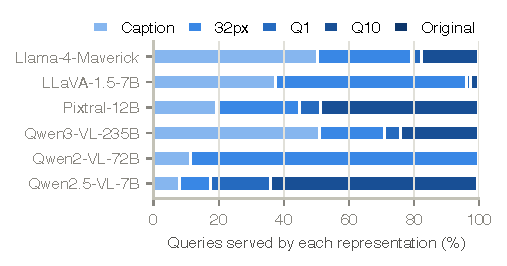
\includegraphics[width=\columnwidth]{figures_v2/selection.pdf}
\caption{Representations selected by \system on FloodNet, by model. Every
model sees the same questions; the mix reflects its measured behavior.}
\label{fig:selection}
\end{figure}

Figure~\ref{fig:selection} shows which representations \system reads. The
caption and the 32-pixel thumbnail together serve 100\% of \mQSevTwo's queries.
They serve 96\% of \mLlava's, 79\% of \mLlama's, and 71\% of \mQThree's. They
serve only 45\% of \mPix's and 18\% of \mQSev's queries, which rely on JPEG Q10.
For every model, the original is read for fewer than 1\% of queries.
% src: generated/selection_distribution.csv

These mixtures have direct placement consequences. Captions and thumbnails
together occupy about 2.4\,KB per image, or 0.04\% of the original's size.
Materializing both at the edge for every asset therefore costs almost nothing.
Averaged across models, it serves 68\% of queries without crossing the
backhaul. JPEG previews add 0.66\,MB per image, or 12\% of the original. They
are worth placing at the edge only for models that select them, such as \mPix
and \mQSev. Originals are read for under 1\% of queries. They can move to a
cold or archive tier with little effect on accuracy. Placement thus depends on
the model mix, so \system optimizes it with its own estimates rather than a
fixed policy.

\phantomsection\label{sec:placement-eval}
\textbf{Placement under capacity sweeps.}
We evaluate the placement advisor in a two-tier setting. All representations are stored
in the cloud. An edge tier holds a fraction of the corpus (7.98\,GB of
originals). Cloud reads follow the recorded uplinks of Table~\ref{tab:trace}.
For each scenario we fit the p95 read latency as $\alpha+b/\beta$
($R^2\ge0.945$). Edge reads take 2\,ms plus $b/(100\,\text{MB/s})$, an assumed
LAN-attached edge server. Image popularity is Zipf(1), and we draw ten random
popularity orders. Every query is routed by Algorithm~\ref{alg:p1} at its
validated $\lambda$, with a 0.25\,s read deadline. A read that misses the
deadline counts as wrong. We compare four placements
(Table~\ref{tab:placement}). \emph{Frequency tiering} fills the edge with the
originals of the most popular images, the usual hot/cold policy. We pair it
either with reading originals, as today's pipelines do, or with \system's
routing. \emph{Size-ordered classes} places whole representation classes in
ascending size. The \emph{placement advisor} (\S\ref{sec:advisor}) fills the edge greedily with the
(image, representation) copies of largest popularity-weighted accuracy gain per
byte. Routing cost is bytes, which are the same on either tier, so an edge copy
helps only when the cloud copy would miss the deadline.
% src: generated_icde/placement_table.tex, generated_icde/numbers.txt
% (scripts/placement_advisor.py; latency fits from VOILA_code trace_sim records)

Frequency tiering of originals answers at most 48.5\% of questions within the
deadline, even with 20\% of the corpus at the edge. Representation selection
matters more than placement. With no edge tier at all, \system's routing
reaches 67.1\%. Placement then closes the remaining gap. With 0.5\% of the
corpus at the edge, the placement advisor reaches 68.5\%. Size-ordered classes need 5\%
to match it. Frequency tiering gains nothing, because \system rarely reads the
originals it caches. The placement advisor's gains come from the two poorest uplinks.
Under the weak-signal trace, 1\% of edge capacity raises accuracy from 62.1\%
to 67.8\%, and the placement advisor uses only 23\,MB of the 80\,MB allowed. Size-ordered
classes reach 63.1\%. On the four better uplinks, every placement reaches the
deadline-free ceiling of 68.9\%. With a 1\,s deadline, placement does not
matter for \system's routing, while frequency tiering of originals reaches at
most 53.2\%. Uniform popularity gives the same ordering.

\begin{table}[t]
\centering
\tableformat
\caption{Deadline-qualified accuracy (\%, 0.25\,s read deadline) by edge
capacity (\% of original bytes). Averaged over six VLMs, six recorded uplinks,
and ten Zipf(1) popularity orders.}
\label{tab:placement}
% src: generated_icde/placement_table.tex
\resizebox{\columnwidth}{!}{%
\begin{tabular}{lrrrrr}
\toprule
Placement & 0\% & 0.5\% & 1\% & 5\% & 20\% \\
\midrule
Frequency tiering, read originals & 0.0 & 19.1 & 24.2 & 37.4 & 48.5 \\
Frequency tiering + \system      & 67.1 & 67.1 & 67.1 & 67.1 & 67.2 \\
Size-ordered classes + \system   & 67.1 & 67.3 & 67.3 & 68.5 & 68.9 \\
Placement advisor + \system      & 67.1 & 68.5 & 68.7 & 68.9 & 68.9 \\
\bottomrule
\end{tabular}}
\end{table}

\subsection{Q5: Robustness, maintenance, and failure}
\label{sec:robust}

\begin{table}[t]
\centering
\tableformat
\caption{Robustness on FloodNet (accuracy \%, per query). Template: entire
question templates held out of training. +FB: unprofiled templates routed to
the validated fallback representation. Struct: TF--IDF removed. Calibration
columns report accuracy / MB per query.}
\label{tab:robust}
% src: generated_icde/robustness_pooled.csv (Main, Template, Delta, +FB);
% generated/robustness_table.tex (Struct); generated/calibration_ablation_table.tex
\resizebox{\columnwidth}{!}{%
\begin{tabular}{lrrrrrcc}
\toprule
Model & Main & Template & $\Delta$ & +FB & Struct & No calib. & Isotonic \\
\midrule
\mLlama   & 68.2 & 59.9 & $-$8.4  & 61.9 & 68.4 & 67.8/0.076 & 68.2/0.086 \\
\mLlava   & 75.7 & 74.3 & $-$1.4  & 74.4 & 76.1 & 75.8/0.001 & 75.7/0.015 \\
\mPix     & 54.3 & 21.3 & $-$33.0 & 50.5 & 53.8 & 54.8/0.224 & 54.3/0.232 \\
\mQThree  & 82.1 & 33.2 & $-$48.9 & 83.2 & 81.1 & 83.2/0.134 & 82.1/0.118 \\
\mQSevTwo & 73.3 & 58.5 & $-$14.7 & 73.9 & 73.4 & 74.0/0.002 & 73.3/0.002 \\
\mQSev    & 69.2 & 63.3 & $-$5.9  & 65.2 & 68.7 & 69.3/0.356 & 69.2/0.354 \\
\bottomrule
\end{tabular}}
\end{table}

\textbf{Unseen question templates are the dominant failure mode.} Holding
out entire question templates reduces per-query accuracy by 1.4--48.9 points,
from 70.5\% to 51.8\% on average (Table~\ref{tab:robust}).
% src: generated_icde/robustness_pooled.csv. Per query, not the unweighted
% mean of the five folds (fold sizes range from 112 to 829 queries).
The loss is concentrated. FloodNet's profiled workload contains 15 distinct
question strings. One of them, ``What is the overall condition of the given
image?'', accounts for 49\% of queries. When it is held out, \mQThree routes it
to the 32-pixel thumbnail and answers 5.7\% correctly. When it is profiled,
\mQThree answers it correctly 96.7\% of the time. Image-grouped folds prevent
visual leakage. They do not guarantee robustness to new phrasings.

\textbf{The fallback recovers the loss.} Routing unprofiled templates to the
best fixed representation on the training folds raises template-holdout
accuracy from 51.8\% to 68.2\%, matching that representation
(Table~\ref{tab:robust}, +FB). Profiled templates are unaffected, so
in-distribution accuracy is unchanged. Detecting novelty by feature distance
does not work here. Every held-out template has TF--IDF cosine similarity of
at least 0.8 to a profiled one. Any threshold that flags the failing template
flags nearly every held-out query. Template novelty is the reliable signal,
because templates recur in analytic workloads like prepared statements.
% src: generated_icde/ood/ood_fallback_*.csv (scripts/ood_audit_fallback.py)

\textbf{Image-grouped protocol on breadth workloads.} We re-ran VQA-v2 and GQA
with image-disjoint folds. Mean accuracy over six models changes from 64.9\% to
63.7\% on VQA-v2 and from 59.6\% to 58.8\% on GQA. Fold standard deviations rise
from under 1 point to 2.9 and 5.8 points. Leakage through shared images or
templates does not explain the results. Generalization to new templates is,
however, less stable. % src: ACL author response to Reviewer HxUU (W4)

\textbf{Cross-model transfer.} An estimator trained on one model's labels can
serve another model without retraining (Table~\ref{tab:xfer}). On VQA-v2 it
stays within 3.4--4.5 points of a target-trained estimator. On GQA it matches
it. An existing estimator can therefore serve an updated model while new
labels accumulate.

\begin{table}[t]
\centering
\tableformat
\caption{Cross-model transfer (accuracy \% @ normalized cost). Zero-shot:
estimator trained on the source model's labels.}
\label{tab:xfer}
% src: ACL author responses to Reviewers HxUU (W3) and kAzo (W3)
\setlength{\tabcolsep}{2.5pt}
\begin{tabular}{llrrr}
\toprule
Data & Source $\rightarrow$ target & Zero-shot & Target-trained & $\Delta$ \\
\midrule
\multirow{3}{*}{VQA-v2} & Qwen2-72B $\rightarrow$ Qwen3-235B & 67.9@30.8 & 71.5@37.4 & $-$3.6 \\
 & Qwen2.5-7B $\rightarrow$ Qwen3-235B & 67.0@30.9 & 71.5@37.4 & $-$4.5 \\
 & Qwen3-235B $\rightarrow$ Qwen2-72B & 61.0@35.6 & 64.4@37.3 & $-$3.4 \\
\midrule
\multirow{3}{*}{GQA} & Qwen2-72B $\rightarrow$ Qwen3-235B & 61.9@26.5 & 59.0@24.3 & +2.9 \\
 & Qwen2.5-7B $\rightarrow$ Qwen3-235B & 60.4@34.3 & 59.0@24.3 & +1.4 \\
 & Qwen3-235B $\rightarrow$ Qwen2-72B & 60.9@29.6 & 60.0@29.0 & +0.9 \\
\bottomrule
\end{tabular}
\end{table}

\textbf{Simple structure carries much of the signal.} Removing TF--IDF and
keeping only structural features changes FloodNet accuracy by at most one
point (Table~\ref{tab:robust}). Under shift between VQA-v2 and GQA, only
49--57\% of the TF--IDF vocabulary overlaps. TF--IDF permutation importance
drops by 62--100\%. Structural features retain most of theirs. Lexical features
are high-capacity but corpus-specific; structural ones transfer.
% src: ICML author response, Reviewer 3DPx

\textbf{Calibration is a model-selection choice.} On FloodNet, isotonic
calibration does not uniformly improve the selected operating point. No
calibration is slightly better for four models (Table~\ref{tab:robust}). On
VQA-v2 and GQA, isotonic calibration reduced cost by 10--25\% relative to
uncalibrated routing at comparable accuracy. For \mPix on VQA-v2, it reduced
expected calibration error from 0.025 to 0.012. % src: ACL Sec. 5, Fig. 3
On FloodNet, the out-of-fold isotonic estimates have expected calibration error
0.021--0.029 (ten bins, all five representations) and Brier score
0.098--0.170, against 0.214--0.248 for a constant predictor. Estimator
training, calibration, operating-point selection, and testing use disjoint
question groups in every fold.
% src: generated_icde/tracker_evidence.txt DESIGN-07 (scripts/tracker_evidence.py);
% VOILA_code scripts/run_all_experiments.py L1457-1474
Calibration is required for P1's subtraction to be meaningful. Which calibrator
works best should be selected on validation data.

\textbf{Estimator family and fair baselines.} We fix calibration and the
optimizer and vary the estimator for \mPix. Gradient boosting, logistic
regression, ridge, and MLP estimators are within 1.6 accuracy points and 5 cost
units of each other on VQA-v2. A fine-tuned BERT regressor in the same pipeline
reaches 66.0\% at cost 42.6 on VQA-v2 and 60.1\% at 35.2 on GQA. Gradient
boosting reaches 64.1\% at 38.8 and 60.5\% at 31.1. BERT thus brings no
consistent improvement, at a much higher estimator cost. Calibrating the
cascade's log-probabilities does not close its gap either. On TextVQA, the
calibrated cascade reaches 71.2\% at cost 26.3, versus 84.8\% at 26.6 for
\system.
% src: ACL Table 14; ACL author responses to SRNH (W2) and xSwT (W4)

\textbf{Objective consistency and the caption tier.} Replacing the legacy
sequential rule with the rule of~\eqref{eq:p1} changes breadth results by
+0.4 accuracy points and +0.7 cost units on average. On FloodNet, the legacy
rule is markedly worse (e.g., 25.8\% vs.\ 54.3\% for \mPix). It under-reads when
gains are non-monotone. Removing the caption tier keeps \system within 2.4
points on VQA-v2, GQA, and FloodNet. It costs 14.4 points on TextVQA. There,
captions are generated from originals and often transcribe scene text. TextVQA
results should therefore be read as depending on that derived view.
% src: ACL author responses to SRNH (W4), xSwT (W3); generated/primary_summary.csv

\begin{table}[t]
\centering
\tableformat
\caption{Failure decomposition on FloodNet (\% of queries). Oracle: answerable
by some representation. Exact: \system picks the cheapest correct one. Under:
wrong although some representation was correct. Over: correct, but with more
bytes than needed. None: no representation is correct.}
\label{tab:failure}
% src: generated/failure_analysis_table.tex
\begin{tabular}{lrrrrr}
\toprule
Model & Oracle & Exact & Under & Over & None \\
\midrule
\mLlama   & 88.6 & 51.8 & 20.3 & 16.4 & 11.4 \\
\mLlava   & 83.7 & 33.6 & 8.0 & 42.1 & 16.3 \\
\mPix     & 79.4 & 40.9 & 25.1 & 13.4 & 20.6 \\
\mQThree  & 90.2 & 59.4 & 8.2 & 22.7 & 9.8 \\
\mQSevTwo & 86.3 & 46.2 & 13.0 & 27.1 & 13.7 \\
\mQSev    & 84.2 & 7.8 & 14.9 & 61.4 & 15.8 \\
\bottomrule
\end{tabular}
\end{table}

\textbf{Where the remaining gap lies.} Table~\ref{tab:failure} separates
reducible from irreducible error. Under-reads affect 8--25\% of queries and
cost accuracy. Better estimates, for example from catalog statistics or
fallbacks, can recover them. Over-reads affect 13--61\% of queries and cost
bytes. Sharper cost discrimination can recover them. Finally, 10--21\% of
queries are answered incorrectly at every representation. Selection cannot fix
them.

\textbf{Overhead.} The saved estimator bundle for one model is 234,666 bytes.
A decision takes 4.12\,ms at the median and 5.32\,ms at p95 on a reference
CPU. Peak process memory is 162\,MB. This is two to four orders of magnitude
below VLM inference (2.4--62.8\,s). It is also far below the access latency of
an original over the recorded uplinks (p50 1.43\,s).
% src: PerCom draft Sec. 6.3; ACL Table 11

%==========================================================================
\section{Discussion}
\label{sec:discussion}

\textbf{When does query-driven selection pay off?} The gains are largest in two
conditions. The workload mixes questions with different evidence needs, and a
model's best fixed representation is large. For \mLlama and \mQThree, the best
fixed input is a 445\,KB preview. \system serves most of their questions from a
caption or thumbnail. It reads 75--80\% fewer bytes at a 1-point accuracy cost.
When a model's best fixed input is already tiny, little is left to save. This
is the case for \mQSevTwo, whose best input is a 2.1\,KB thumbnail. There, the
optimizer correctly converges to almost the same policy.

\textbf{Estimates as optimizer statistics.} \system's success estimators play
the role that cardinality estimates play in a relational optimizer. They price
alternatives that the optimizer never executes. Their errors turn into plan
regret (Proposition~\ref{prop:regret}). The same operational practices apply.
Estimates must be refreshed when the workload drifts. Template holdout is the
analogue of a stale histogram. Estimates must be validated on data the
optimizer did not train on. They need a conservative fallback
for queries they were never fitted to, as an optimizer falls back to a
safe plan when statistics are missing.

\textbf{Accuracy floors as service-level objectives.} The validation rule keeps
accuracy within 95\% of the best fixed representation. This is a contract, not
a constant. A medical archive would raise it. A best-effort photo search would
lower it. Because the estimates are probabilities, changing the contract
changes only the operating point. The estimators stay the same.

\textbf{Composition.} Representation selection composes with model routing,
which chooses the model after the input is fixed. It also composes with
in-model token reduction~\cite{cai2024matryoshka,chen2024fastv}, which shrinks
the computation on the bytes that were read. A joint optimizer over
(representation, model) pairs is a natural extension. It would require success
estimates for every pair.

\textbf{Data minimization.} Reading a caption or thumbnail instead of an
original means fewer bytes leave the storage tier. Images often contain
incidental personal information. Selecting the least detailed sufficient
representation is then a data-minimization measure as well as a cost
optimization.

%==========================================================================
\section{Related Work}
\label{sec:related}

\textbf{Visual data management.} Video and visual DBMSs store multiple physical
representations and choose cheap ones to serve queries. VStore selects storage
and consumption formats for video analytics pipelines~\cite{xu2019vstore}. VSS
stores and reuses multiple physical video representations~\cite{haynes2021vss}.
TASM stores tiles so that queries read only regions of
interest~\cite{daum2021tasm}. LightDB optimizes declarative queries over VR
video~\cite{haynes2018lightdb}. These systems choose among representations that
satisfy an explicitly stated format or a profiled vision pipeline. \system
addresses the case where the consumer is a general VLM answering a free-form
question. The required representation must then be inferred from the question
and the model.

\textbf{ML inference in query processing.} NoScope, BlazeIt, probabilistic
predicates, and TASTI reduce the cost of neural predicates and aggregates over
video and unstructured data~\cite{kang2017noscope,kang2020blazeit,
lu2018probabilistic,kang2022tasti}. They use cheap proxies, indexes, and
sampling. Smol jointly optimizes preprocessing and inference, including
low-resolution inputs~\cite{kang2020smol}. LLM-powered engines such as LOTUS,
Palimpzest, ThalamusDB, and CAESURA optimize semantic operators and model
choices over multimodal data~\cite{patel2024lotus,liu2025palimpzest,
jo2024thalamusdb,urban2024caesura}. These systems decide after data is local,
or by running models on it. \system decides which stored representation to read
before reading. It can supply its choice to any of them.

\textbf{Approximate query processing and physical design.} BlinkDB maintains
samples of different sizes. It selects one per query to meet error and latency
bounds~\cite{agarwal2013blinkdb}. \system analogously maintains
representations of different fidelity. It selects one per query against an
estimated accuracy, with VLM correctness as the error model. Placing
representations across tiers is a physical-design problem, like
view and index selection~\cite{harinarayan1996cubes,chaudhuri1997autoadmin}.
\system's estimates serve as its cost model.

\textbf{Routing and cascades.} FrugalML, FrugalGPT, RouteLLM, and hybrid routing
select among models or APIs for a given input~\cite{chen2020frugalml,
chen2023frugalgpt,wang2024routellm,ding2024hybrid,shnitzer2023large}.
Early-exit methods shorten computation~\cite{zhou2020bert,
schuster2022confident}. These methods optimize how an available input is
processed. They can follow \system's selection.

\textbf{Query difficulty and value of information.} Pre-retrieval query
performance prediction estimates retrieval quality from query features
alone~\cite{zhao2008predicting,hauff2008improved,mothe2005linguistic}. VQA
analyses show that question type predicts difficulty~\cite{kafle2017analysis,
agrawal2018dont}. Value-of-information and cost-sensitive acquisition decide
whether evidence is worth its cost~\cite{bilgic2011value,karkkainen2019cost,
kossen2022active}. \system applies these ideas to the representations of an
identified asset. Model-specific correctness is the value, and catalog-priced
access is the cost. Adaptive resolution inside VLMs~\cite{cai2024matryoshka,
chen2024fastv,kimhi2025cares} reduces computation on an image already read. It
is complementary.

%==========================================================================
\section{Limitations}
\label{sec:limits}

\textbf{The question is a partial signal.} The same question can require
different detail for different images, such as a large versus a distant
object, and compound or conditional questions blur the signal. Unseen
templates are the main risk (\S\ref{sec:robust}). The fallback recovers
best-fixed accuracy but forgoes \system's savings until the new template is
profiled, and it needs recurring templates. On open-ended workloads (69--82\%
unseen strings), \system still cuts cost by 65--73\% (Table~\ref{tab:breadth}),
but guarding against harmful novelty there would need a semantic novelty
signal. Conditioning the estimators on catalog features such as caption text,
and conformal novelty tests, are natural next steps.
% src: generated_icde/template_coverage.txt (69--82%, question-level 5-fold, may not match the breadth runs' exact folds); 65--73%: tab:breadth

\textbf{Discrete, profiled representations.} \system chooses among materialized
representations and needs correctness labels per model; a new representation
or model requires profiling only for the new component. Online profiling from
production feedback could replace the offline labeling step.

\textbf{Measured costs on one workload.} Measured bytes and network traces are
reported on FloodNet; the breadth datasets use a tier-weighted cost model. The
trace experiment simulates serialization over recorded delivery opportunities
and omits transport-protocol dynamics.

\textbf{Derived captions.} Captions are generated from originals at ingestion,
and their one-time cost is excluded from per-query accounting. On OCR-heavy
data, they carry information that low-resolution images do not. Deciding which
representations to materialize, not only where, extends P3.

\textbf{English questions.} Features and question-type rules target English.
Multilingual queries require new profiling data.

%==========================================================================
\section{Conclusion}

A VLM query over image data does not have to read the original. \system treats
the choice of representation as an optimizer decision taken before any pixel is
read. It uses calibrated, model-specific estimates of answer correctness,
derived from the question text. It prices representations with a catalog of
where each one lives and what it costs. On a disaster-response workload, it is
as accurate on average as the best fixed representation chosen on validation
data while reading 84\% fewer bytes, and it nearly doubles the share of
questions answered correctly within one second. The same estimates allocate
shared workload budgets and, in a two-tier simulation, guide which
representations an edge tier should hold. The main failure case is question
templates absent from profiling. A template fallback contains it on templated
workloads. Open-ended workloads mark where data systems will need richer
evidence about what a query needs, still without reading pixels.
% src: as abstract (generated/main_results_table.tex, generated/paired_bootstrap.csv)

\section*{Acknowledgement of AI-Generated Content}
Claude Code and Codex were used for grammar and editorial assistance in
Sections~I--X of this paper. They also assisted with writing and revising the
VOILA implementation and experimental scripts underlying Sections~III--VII;
the tools were not used to generate experimental measurements. Every line of
AI-generated code was reviewed by at least one author, and the authors take
responsibility for the correctness and originality of the paper, code, and
results.

\bibliographystyle{IEEEtran}
\bibliography{example_paper,systems_refs}

\end{document}
